\documentclass[../draft.tex]{subfiles}

\begin{document}
    \chapter{Theory}
    In the first part of this chapter, we define the flow functions and in the second part we discuss the time complexity of taint analysis specificly hightlighting differences between forward and backward analysis.

    \section{Flow Functions}\label{s:flowfunctions}
    We describe the behavior of the flow functions based on the Jimple language and define semi-formal rules analogous to the publication\cite{Arzt2017PhD} on \textsc{FlowDroid}. These rules only focus on the base control-flow, we describe flows for additional language features such as arrays and exceptions later more informal in \autoref{s:rules}. Note that traversing the interprocedural control-flow graph backwards means call edges are now return edges and vice versa. 

    \subsection{Normal Flow}\label{s:normalflow}
    Normal flow functions handle every statement that does not contain an \code{InvokeExpr} and assignments are always explicit in Jimple.
    For the base cases, new taint are only produced at \code{AssignStmt}s. We skip over \code{IdentityStmt} even though they also assign values such as the \code{this} reference or the parameters to locals. The Return Flow Function is responsible for mapping all parameters back into the callee and the return edge is after the \code{IdentityStmt}s.

    Now, lets consider the current statement is an \code{AssignStmt}. It consists of a variable, either a reference or a local, on the left side and an expression on the right side. The assigment has the structure $x.f^n \leftarrow y.g^m$ with $n,m \in \{0,1\}$ modelling a possible field reference. As taints may have an access path of an arbitrary length, we denote the rest as $h^k$.\footnote{$h^k$ is a $k$-length access path, not $k$-times the same field reference} Jimple also ensures only one field dereference per statement which Arzt chose not to represent in the semi-formal definitions. 

    In the first case, we look at exact matches. Either we have an assignment with a local ($n=0$) or a field dereference ($n=1$). For both, the base variable needs to match. For the latter, also the first field of the access path has to match the field dereference.
    The first field dereference is removed from the taint and the remaining access path is copied to the newly created taint. The incoming taint is killed because it received the worthwhile information at this statement.
    \begin{itemize}
        \item[] \textbf{Rule 1:} An incoming taint $T = x.f^n.h^k$ with $k \geq 0$ produces the outflowing taint set $\left\{y.g^m.h^k\right\}$.
    \end{itemize} 
    Rule 1 work likewise with a wildcard appended after $h^k$. Similiary to the rest access path $h^k$, it is copied to the right side.

    Next, we need a rule for the case the field dereference $f$ is included in $*$. Recall \autoref{s:ap}, symbolic access paths can also be $k$-limited to speedup the analysis and they are $k=5$-limited in \textsc{FlowDroid} by default. Thus, we might encounter a taint with no field dereferences and a wildcard appended. In this case, just the base needs to match. But this time, the left side is kept alive because we can not reason which field is tainted due to the cut-off approximation.
    \begin{itemize}
        \item[] \textbf{Rule 2:} An incoming taint $T = x.*$ with $k \geq 0$ produces the outflowing taint set $\left\{y.g^m.*, T\right\}$.
    \end{itemize} 

    Lastly, we could also observe a taint on the right side. In this case, we simply apply the identity, so propagate the taint over the statement. This case also gets important later when we consider aliasing in \autoref{s:aliasing}.
    \begin{itemize}
        \item[] \textbf{Rule 3:} An incoming taint $T = y.g^m.h^k$ with $k \geq 0$ produces the outflowing taint set $\left\{T\right\}$.
        \item[] \textbf{Rule 4:} An incoming taint $T = y.*$ produces the outflowing taint set $\left\{T\right\}$.
    \end{itemize}

    Whenever a taint neither matches on the left nor on the right side, we also perform the identity as the statement does not touch the contents of the tainted variable.  

    \subsection{Call Flow}
    The Call Flow Function and subsequently also Return and Call TO Return Flow Function is applied whenever a statements contains an \code{InvokeExpr}.
    For call statements without assignments, we have statements of the structure $o.m(a_0, ..., a_n)$ with $n \in \mathbb{N}$. $a_i$ denotes the $i$-th argument, $p_i$ the $i$-th parameter and $c$ the class instance of the callee's base object.

    When we encounter a tainted argument in the caller, the taint needs to go through the callee. Java uses pass-by-value, so the arguments are copied into the callee. Thus, for primitives, the value is copied and pushed onto the stack and for reference types, the pointer to the object is copied into the callee. In the second case, if only the base reference is tainted but nothing more ($k=0$ and no wildcard), the callee can only access and overwrite the reference saved in the parameter on the stack but not change the data of the object on the heap. 
    Due to the backwards direction, we know the update which tainted the primitive or reference without field dereferences can not be inside the callee. This gets more clear when we get specific to Java's types. Primitives do not have fields and strings are immutable\footnote{The special handling of strings results in transparent fields, e.g. we can treat strings as if they were primitives in this case.}. Consider the example in \autoref{lst:primret}. On the left, we use the built-in String type. In line 2, \code{str} is copied into \code{callee}. At this point, \code{main} holds the \code{str} with the value "42" but pointing to another memory location than \code{str} in \code{callee}\footnote{The JVM might only set a copy-on-write flag on \footnotecode{str} in \footnotecode{callee} and point it to the same location as \footnotecode{str} in \footnotecode{main} to save memory. At least right before the update happens, it is guranteed that the variable points to a different location.}. Thus, \code{main} carries on with the original value of \code{str} no matter what \code{callee} writes to \code{str}. In contrast on the right, the callee can update the field on the heap and therefore, the taint needs to be propagated into the callee to find the leak. Conclusively, $k$ needs to be greater than $0$.

    \begin{figure}[t]
        \centering
        \begin{subfigure}[b]{0.45\textwidth}
            \centering
            \begin{adjustbox}{max width=\columnwidth}
                \begin{lstlisting}[gobble=20]
                    void main() {
                        String str = "42";
                        callee(str);
                        sink(str); // no leak
                    }
            
                    void callee(String str) {
                        str = source();
                    }
                \end{lstlisting}
            \end{adjustbox}
            \caption{Taint Without Fields}
        \end{subfigure}
        \qquad
        \begin{subfigure}[b]{0.45\textwidth}
            \centering
            \begin{adjustbox}{max width=\columnwidth}
                \begin{lstlisting}[gobble=20]
                    void main() {
                        SomeObject o = new SomeObject();
                        callee(o);
                        sink(o.str); // leak
                    }
            
                    void callee(SomeObject o) {
                        o.str = source();
                    }
                \end{lstlisting}
            \end{adjustbox}
            \caption{Taint With Fields}
        \end{subfigure}
        \caption{Call Flow Example}
        \label{lst:primret} 
    \end{figure}

    \begin{itemize}
        \item[] \textbf{Rule 1:} An incoming taint $T=a_i.h^k$ with $k > 0 \land 0 \leq i \leq n$ produces the outflowing taint set $\left\{p_i.h^k\right\}$.
        \item[] \textbf{Rule 2:} An incoming taint $T=a_i.*$ with $0 \leq i \leq n$ produces the outflowing taint set $\left\{p_i.*\right\}$.
    \end{itemize}

    A non-static callee can also access instance fields of the base object. When we observe a tainted base object, the taint also needs to flow through the callee. The tainted object transforms into a $\mathit{this}$ reference. In Java \code{this} is used to  reference the current instance the method operates on.
    \begin{itemize}
        \item[] \textbf{Rule 3:} An incoming taint $T=o.h^k$ with $k \geq 0$ produces the outflowing taint set $\left\{\mathit{this}_c.h^k\right\}$. 
        \item[] \textbf{Rule 4:} An incoming taint $T=o.*$ produces the outflowing taint set $\left\{\mathit{this}_c.*\right\}$.
    \end{itemize}
    
    Static fields are a special case. Their scope is the whole program and thus, are always visible in the callee. The taint is untouched as the access path to those is the same everywhere.
    \begin{itemize}
        \item[] \textbf{Rule 5:} An incoming taint $T = S.f.h^k$ with $k \geq 0$ produces the outflowing taint set $\left\{T\right\}$.
    \end{itemize}

    In Jimple, an \code{AssignStmt} can also consist of a \code{Local} on the left side and an \code{InvokeExpr} on the right side. The structure of the statement is in this case $x \leftarrow o.m(a_0,...,a_n)$. $r_i$ denotes a return value. $m$ is the number of return statements in the callee. If we observe such a statement and the left side is tainted as well, we need to map the returned value back into the callee. Now, methods can have multiple return statements and as we traverse the reversed interprocedural control-flow graph, there are multiple edges to go with. We can not reason which return statement is the right one, so we need to taint the operand of every return statement in the callee.
    \begin{itemize}
        \item[] \textbf{Rule 6:} An incoming taint $T = x.h^k$ with $k \geq 0$ produces the outflowing taint set $\left\{r_i.h^k \mid 0 \leq i < m \right\}$. 
    \end{itemize}

    Unlike at normal flows, we kill all taints not matching any of the rules. In the case of a taint being out of the callee's scope, the Call To Return flow function propagates the taint over the statement.

    \subsection{Return Flow}
    Reaching the end of a method, the taints need to be mapped back into the caller. The statement we consider is of the structure $o.m(a_0, ..., a_n)$ with $n \in \mathbb{N}$. Again, $a_i$ denotes the $i$-th argument, $p_i$ the $i$-th parameter and $c$ the class instance.

    The first rule matches rule 1 and 2 of call flow: map all parameters back into the caller. In contrast to call flow, this time we also map primitives and strings back into the caller because the contents of the variable were copied from the caller's argument into the callee.
    \begin{itemize}
        \item[] \textbf{Rule 1:} An incoming taint $T = p_i.h^k$ with $k \geq 0 \land 0 \leq i \leq n$ produces the outflowing taint set $\{a_i.h^k\}$.
    \end{itemize}

    The $\mathit{this}$ reference also needs to be mapped back into the caller.
    \begin{itemize}
        \item[] \textbf{Rule 2:} An incoming taint $T = \mathit{this}_c.h^k$ with $k \geq 0$ produces the outflowing taint set $\{o.h^k\}$. 
        \item[] \textbf{Rule 3:} An incoming taint $T = \mathit{this}_c.*$ with $k \geq 0$ produces the outflowing taint set $\{o.*\}$.
    \end{itemize}
    
    Tainted static fields are also mapped back untouched. This is the same as rule 5 of the Call Flow.
    \begin{itemize}
        \item[] \textbf{Rule 4:} An incoming taint $T = S.h^k$ with $k \geq 0$ produces the outflowing taint set $\{T\}$. 
    \end{itemize}
    
    Again, taints not matching any rule are killed. For example, this is the case when returning from a method and the variable is not in the scope of the caller.

    \subsection{CallToReturn Flow}
    The statement structure is $o.m(a_0, ..., a_n)$ with $n \in \mathbb{N}$. $a_i$ denotes the $i$-th argument.

    A taint is not in scope of the callee if it is not static and neither matches an argument nor the base object the method is called on. Such a taint is not matched inside Call Flow and needs to be propagated over the call statement.
    \begin{itemize}
        \item[] \textbf{Rule 1:} An incoming taint $T = x.h^k$ with $k \geq 0 \land \left(\forall i \in [0, n] \cap \mathbb{N}: a_i \neq x\right) \land x \neq o \land x \notin \mathit{StaticVariables}$ produces the outflowing taint set $T = \{t\}$. 
    \end{itemize}

    Consider again the left side of \autoref{lst:primret}. In line 3, the taint is in the kill set of Call Flow. But as we want to preserve the taint after the call, we need to propagate the taint over the call statement in such cases. 
    \begin{itemize}
        \item[] \textbf{Rule 2:} An incoming taint $T = a_i$ with $0 \leq i \leq n$ produces the outflowing taint set $\{T\}$. 
    \end{itemize}
        
    Like in Call and Return Flow, here we also kill taints which do not match any of these rules.
    
    \section{Complexity of Data Flow Analysis}\label{s:complexity}
    IFDS has a time-complexity of $O(E \cdot D^3)$. The edges in the control-flow graph are set by the to-be-analyzed app. The domain depends on the tainted variables observed by the IFDS analysis. The number of taint propagations should directly correlate to the runtime and depends on two factors: the lifetime of taints and the number of taints. Both factors are influenced by the search direction which we will explain in the following paragraphs.

    \begin{figure}[ht]
        \centering
        \begin{adjustbox}{max width=\textwidth}
            \begin{lstlisting}[gobble=16]
                String returnParam(int i, String s1, String s2, String s3) {
                    if (i == 1)
                        return s1;
                    else if (i == 2)
                        return s2;
                    else if (i == 3)
                        return s3;
                    else
                        return "default";
                }
            \end{lstlisting}    
        \end{adjustbox}
        \caption{Branching Factor Example}
        \label{lst:branching}
    \end{figure}

    First, we take a look at the is the branching factor. The branching factor describes the number outgoing edges from a node. A smaller branching factor is favorable.   
    Think of binary operator expression such as \code{int c = a + b;}, backwards we can not argue which operand is responsible for the tainted output and thus proceed with both operands tainted. The same restriction is present in rule 5 of Call Flow which describes how the returned value is mapped back into the callee. This time the branching factor can be even larger. As an example, in \autoref{lst:branching} is a method which conditionally returns one of its parameters and is part of the leak path. Lets assume the returned value of a call to \code{returnParam()} is tainted. Backwards, every returned operand is tainted and later on mapped according to Return Flow rule 2 back into the caller. Thus, the IFDS algorithm ends up with a summary $\mathit{retVal} \rightarrow \{s1, s2, s3\}$. Forwards, a tainted parameter is mapped into the callee and later on returned to the caller resulting in a summary $sX \rightarrow \mathit\{\mathit{retVal}, sX\}$ with $X \in \{1,2,3\}$. Such cases favors forwards analysis.

    In contrast, a strict right-to-left flow favors backward analysis as backwards taints are killed more often due to a stronger overwrite rule meaning a shorter lifetime per taint. In \autoref{tikz:rtol} is such a right-to-left flow displayed. Forwards, the right hand side is always kept alive because it still holds the tainted value below the statement and could be leaked. 
    This is not the case when searching backward. When the incoming taint is on the left side, the statement is the update which is responsible for tainting. Above this, the contents of the left side is uninteresting. With aliasing, this advantage is not as present.

    \begin{figure}[ht]
        \centering
        \begin{subfigure}[b]{0.45\textwidth}
            \centering
            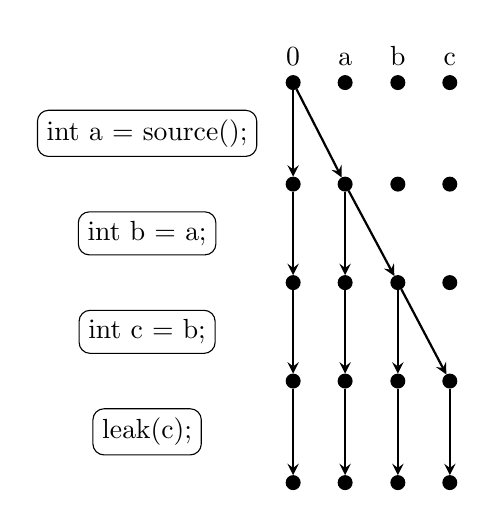
\begin{tikzpicture}[auto, 
                s/.style={draw, rounded corners},
                v/.style={draw, fill=black, circle, inner sep=0pt, minimum size=5pt},
                every node/.style={align=center},
                every matrix/.style={ampersand replacement=\&,column sep=0.25cm,row sep=.25cm},
                vto/.style={->, >=stealth, thick}]
                \matrix {
                    \& \node[v, label={0}] (zero1) {}; \& \node[v, label={a}] (a1) {}; \& \node[v, label={b}] (b1) {}; \& \node[v, label={c}] (c1) {};\\
                    \node[s] (s1) {\smallcode{int a = source();}}; \& \& \& \&\\
                    \& \node[v] (zero2) {}; \& \node[v] (a2) {}; \& \node[v] (b2) {}; \& \node[v] (c2) {};\\
                    \node[s] (s2) {\smallcode{int b = a;}}; \& \& \& \&\\
                    \& \node[v] (zero3) {}; \& \node[v] (a3) {}; \& \node[v] (b3) {}; \& \node[v] (c3) {};\\
                    \node[s] (s3) {\smallcode{int c = b;}}; \& \& \& \&\\
                    \& \node[v] (zero4) {}; \& \node[v] (a4) {}; \& \node[v] (b4) {}; \& \node[v] (c4) {};\\
                    \node[s] (s4) {\smallcode{leak(c);}}; \& \& \& \&\\
                    \& \node[v] (zero5) {}; \& \node[v] (a5) {}; \& \node[v] (b5) {}; \& \node[v] (c5) {};\\
                };
                
                \draw[vto] (zero1) -- (zero2);
                \draw[vto] (zero2) -- (zero3);
                \draw[vto] (zero3) -- (zero4);
                \draw[vto] (zero4) -- (zero5);
        
                \draw[vto] (zero1) -- (a2);
                \draw[vto] (a2) -- (a3);
                \draw[vto] (a3) -- (a4);
                \draw[vto] (a4) -- (a5);
                \draw[vto] (a2) -- (b3);
                \draw[vto] (b3) -- (b4);
                \draw[vto] (b4) -- (b5);
                \draw[vto] (b3) -- (c4);
                \draw[vto] (c4) -- (c5);
            \end{tikzpicture}
            \caption{Forwards}
            \label{tikz:rtol_a}
        \end{subfigure}
        \qquad
        \begin{subfigure}[b]{0.45\textwidth}
            \centering
            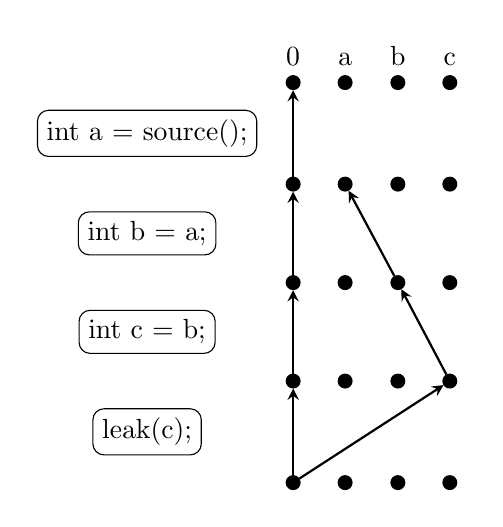
\begin{tikzpicture}[auto, 
                s/.style={draw, rounded corners},
                v/.style={draw, fill=black, circle, inner sep=0pt, minimum size=5pt},
                every node/.style={align=center},
                every matrix/.style={ampersand replacement=\&,column sep=0.25cm,row sep=.25cm},
                vto/.style={->, >=stealth, thick}]
                \matrix {
                    \& \node[v, label={0}] (zero1) {}; \& \node[v, label={a}] (a1) {}; \& \node[v, label={b}] (b1) {}; \& \node[v, label={c}] (c1) {};\\
                    \node[s] (s1) {\smallcode{int a = source();}}; \& \& \& \&\\
                    \& \node[v] (zero2) {}; \& \node[v] (a2) {}; \& \node[v] (b2) {}; \& \node[v] (c2) {};\\
                    \node[s] (s2) {\smallcode{int b = a;}}; \& \& \& \&\\
                    \& \node[v] (zero3) {}; \& \node[v] (a3) {}; \& \node[v] (b3) {}; \& \node[v] (c3) {};\\
                    \node[s] (s3) {\smallcode{int c = b;}}; \& \& \& \&\\
                    \& \node[v] (zero4) {}; \& \node[v] (a4) {}; \& \node[v] (b4) {}; \& \node[v] (c4) {};\\
                    \node[s] (s4) {\smallcode{leak(c);}}; \& \& \& \&\\
                    \& \node[v] (zero5) {}; \& \node[v] (a5) {}; \& \node[v] (b5) {}; \& \node[v] (c5) {};\\
                };
        
                \draw[vto] (zero5) -- (zero4);
                \draw[vto] (zero4) -- (zero3);
                \draw[vto] (zero3) -- (zero2);
                \draw[vto] (zero2) -- (zero1);
        
                \draw[vto] (zero5) -- (c4);
                \draw[vto] (c4) -- (b3);
                \draw[vto] (b3) -- (a2);
            \end{tikzpicture}      
            \caption{Backwards}
            \label{tikz:rtol_b}  
        \end{subfigure}
        \caption{Right-to-Left Order}
        \label{tikz:rtol}
    \end{figure}

    We already mentioned the global scope of static field taints in the last section. This global scope is an issue in both directions as a static field can be accessed anywhere in the code and therefore need to be propagated into every method. Unless the static taint is overwritten, they traverse the whole interprocedural control-flow graph. \textsc{FlowDroid} already applies an optimization and looks ahead in methods and skips methods in which the static field is not used. Still, static fields stay an issue \cite{Arzt2017PhD}.

    Now, it would be beneficial to be able to decide which direction is the best before analyzing an app. An obvious choice for a clue would be the ratio of sources and sinks. If one is much less than the other, we could argue less taints to start with should also lower the taint propagations. 
    Likewise, Lerch et al. claims in their work that much less sources than sinks are advantageous for a backward-directed search \cite{Lerch2014}. 
    Sadly, it is not as easy to just say less starting taints mean less runtime. Arzt's evaluation of \textsc{FlowDroid} has shown no correlation between the number of sources and the runtime \cite{Arzt2017PhD}. This results is probably owed to the unpredictable lifetime of taints.
    As a part of this work, we evaluate whether the favorable search direction can be decided at least on the same app in \autoref{s:realworld}.

    In general, we can not really predict the lifetime of taints before actually analyzing the app. But in special cases of application, this might be given. Think of a case where sanitization methods\footnote{Sanitization methods are run against user input to ensure the input is safe to be processed.} are in use. Depending on the use case, it might be possible to deduce a proximity between sanitization methods and sources or sinks. Whenever this is possible, there should be a clear favor for one direction due to the lower lifetime of the taints. 

    Summarized, we discussed cases where one direction seems favorable but no generalized statement can be made on which analysis direction is better. Further, most of the influencing factors are most influencing factors depend on the app and thus, at most a favorable direction can be determined for a single app.
\end{document}